\section{Непараметрическое восстановление плотности}

Пусть $ X^\ell = (x_i)_{i = 1}^\ell $ --- выборка из распределения с обобщённой
плотностью $p$. Будем строить \emph{непараметрическую} модель для нахождения оценки
плотности $\hat{p}$.

\subsection*{Оценки одномерных плотностей}
В \textbf{дискретном случае} $x_i \in D,\,|D| \ll \ell$ имеем гистограмму частот
\begin{equation*}
\hat{p}(x) = \frac{1}{\ell}\sum_{i = 1}^\ell [x_i = x].
\end{equation*} 
При этом из усиленного закона больших чисел для всех $x$ получим
$ \hat{p}_\ell(x)~\asto~p(x) $ при $ \ell \to \infty $.

Пусть теперь $X^\ell$ --- выборка из \textbf{абсолютно непрерывного}
распределения с плотностью $p$. В этом случае, обозначая за $P[a,b]$
вероятностную меру отрезка имеем
\begin{equation*}
p(x) = \lim_{h \to 0}\frac{P[x - h, x + h]}{2h}.
\end{equation*}
Заменяя вероятность на её эмпирическую оценку, получим
\emph{эмпирическую оценку плотности по окну ширины $h$}.
\begin{align*}
\hat{p}_h(x)
  &= \frac{1}{2h\ell}\sum_{i = 1}^\ell [|x_i - x| < h]\\
  &= \frac{1}{h\ell}\sum_{i = 1}^\ell \frac{1}{2}\left[\frac{|x_i - x|}{h} < 1\right].
\end{align*}

Применим теперь идею метода окна Парзена и формулы Надарая-Ватсона. Обобщим
слагаемое $ \frac{1}{2}\frac{|x_i - x|}{h} < 1 $ с помощью \emph{ядра} $K(r)$,
удовлетворяющего четырём свойствам
\begin{itemize}
\item чётность,
\item неотрицательность,
\item неубывание при $r > 0$,
\item условие нормировки: $ \int K(r) \dd{r} = 1$.
\end{itemize}
Таким образом, мы получим \emph{оценку Парзена-Розенблатта} или
\emph{ядерную оценку плотности (Kernel Density Estimate, KDE)}
\begin{equation*}
\hat{p}_h(x)
  = \frac{1}{h\ell}\sum_{i = 1}^\ell K\left(\frac{|x_i - x|}{h}\right).
\end{equation*}

\subsection*{Оценки многомерных плотностей}
Если объект $x_i$ описывается $n$ независимыми признаками $f_j: X \to \R$,
получаем оценку плотности
\begin{equation}
\hat{p}_{h_1 \ldots h_n}(x)
  = \frac{1}{\ell}\sum_{i = 1}^\ell
    \prod_{j = 1}^n \frac{1}{h_j} K\left(\frac{|f_j(x_i) - x|}{h_j}\right).
\label{kde:features}
\end{equation}

Оценку также можно обобщить, если $ (X, \rho) $ --- метрическое пространство.
Определив нормировочный множитель
$V(h) = \int_X K\left(\frac{\rho(x_i, x)}{h}\right) \dd{x}$, получим
\begin{equation}
\hat{p}_h(x)
  = \frac{1}{\ell V(h)}\sum_{i = 1}^\ell K\left(\frac{\rho(x_i, x)}{h}\right).
\label{kde:metric}
\end{equation}
\subsection*{Виды ядер}

Наиболее распространённые в использовании ядра представлены на Рис.~\ref{kde:kernels}.
\begin{itemize}
\item $E(r) = \frac{3}{4}(1 - r^2)[|r| < 1]$ --- \emph{ядро Епанечникова};
\item $Q(r) = \frac{15}{16}(1 - r^2)^2 [|r| < 1]$ --- \emph{квартичеcкое ядро};
\item $T(r) = (1 - |r|) [|r| < 1]$ --- \emph{треугольное ядро};
\item $G(r) = \frac{1}{\sqrt{2\pi}} \exp(-\frac{1}{2} r^2)$ --- \emph{гауссовское ядро};
\item $\Pi(r) = \frac{1}{2} [|x| < 1]$ --- \emph{прямоугольное ядро}.
\end{itemize}

\begin{figure}[h]
\centering
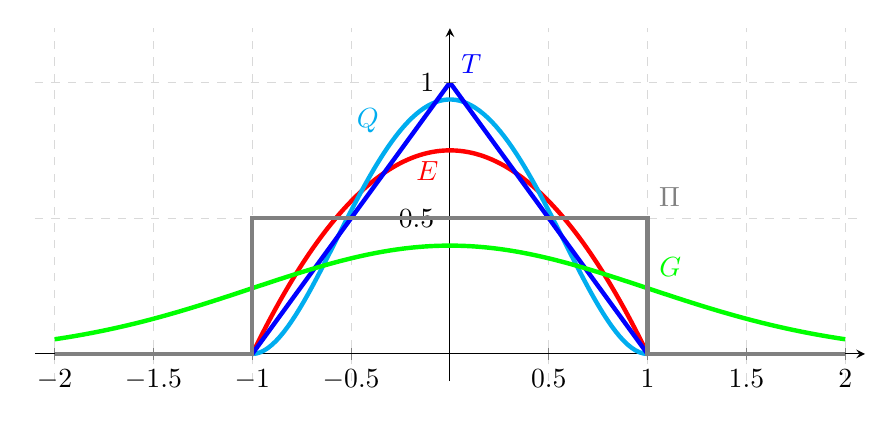
\begin{tikzpicture}
\begin{axis}[
  axis lines=center,
  width=\linewidth,
  height=0.5\linewidth,
  grid=major,
  grid style={dashed, gray!30},
  xmin=-2.1,
  xmax=2.1,
  ymin=-0.1,
  ymax=1.2
]

\addplot[domain=-1:1,samples=100,ultra thick,red] {3 / 4 * (1 - x^2)}
  node [pos=0.5, below left] {$E$};
\addplot[domain=-2:-1,samples=2,ultra thick,red] {0};
\addplot[domain=1:2,samples=2,ultra thick,red] {0};

\addplot[domain=-1:1,samples=100,ultra thick,cyan] {15 / 16 * (1 - x^2)^2}
  node [pos=0.375, above left] {$Q$};
\addplot[domain=-2:-1,samples=2,ultra thick,cyan] {0};
\addplot[domain=1:2,samples=2,ultra thick,cyan] {0};

\addplot[domain=-1:1,samples=100,ultra thick,blue] {1 - abs(x)}
  node [pos=0.5, above right] {$T$};
\addplot[domain=-2:-1,samples=2,ultra thick,blue] {0};
\addplot[domain=1:2,samples=2,ultra thick,blue] {0};

\addplot[domain=-2:2,samples=200,ultra thick,green] {1/sqrt(2 * pi) * e^(- 1 / 2 * x^2)}
  node [pos=0.75, above right] {$G$};

\addplot+[const plot, no marks, ultra thick, gray] coordinates {(-2, 0) (-1, 0) (-1, 1/2) (1, 1/2) (1, 0) (2, 0)}
  node [pos=0.7, above right] {$\Pi$};

\end{axis}
\end{tikzpicture}
\caption{Наиболее распространённые виды ядер.}\label{kde:kernels}
\end{figure}

Заметим, что в случае гауссовского ядра
формулы~\eqref{kde:features}~и~\eqref{kde:metric} совпадают.

Отметим также, что ядро Епанечникова называют также \emph{оптимальным},
поскольку оценка, полученная с его помощью даёт минимум функции риска
\[
J(K) = \int_{-\infty}^{+\infty} \E[ (\hat{p}_h(x) - p(x))^2 ] \dd{x}.
\]
Прочие ядра имеют следующие асимптотические значения функционала $J(K)/J(E)$ при
$\ell \to \infty$:
\begin{center}
\begin{tabular}{|l|l|c|}
\hline
\textbf{Ядро} $K(r)$ & \textbf{Степень гладкости} & $J(K)/J(E)$ \\
\hline
Епанечникова & $\hat{p}_h'$ разрывна & 1.000\\
Квартическое & $\hat{p}_h''$ разрывна & 0.995\\
Треугольное & $\hat{p}_h'$ разрывна & 0.989\\
Гауссовское & $\hat{p}_h\in C^\infty$ & 0.961\\
Прямоугольное & $\hat{p}_h$ разрывна & 0.943\\
\hline
\end{tabular}
\end{center}
Таким образом, поскольку ядра мало отличаются по качеству, на практике обычно
используется гауссовское ядро, в силу удобства вычислений с ним.

\subsection*{Ширина окна}
\begin{wrapfigure}{R}{0.3\textwidth}
\includegraphics[width=0.3\textwidth]{kde_bandwidth.png}
\caption{Зависимость оценки плотности от ширины окна.}\label{kde:bandwidth}
\end{wrapfigure}

На Рис.~\ref{kde:bandwidth} показаны оценки Парзена-Розенблатта с шириной окна
$h=0.05$ (красный график), $h=0.337$ (чёрный график) и $h=2$ (зелёный график)
для 100 точек из стандартного нормального распределения (серый график). При
малых $h$ заметно переобучение, при больших --- недообучение. Таким образом,
качество восстановления плотности в основном зависит от ширины окна.

\newpage
\subsection*{Задачи}

\begin{task}
Пусть $X^\ell$ --- выборка из равномерного на отрезке $[0,1]$ распределения.
Будем использовать прямоугольное ядро и $0 < h < \frac{1}{2}$. Найдите
$\tilde{p}_h(x) = \E[\hat{p}_h(x)]$. Как влияет параметр $h$ на точность
приближения в среднем?
\end{task}

\begin{solution}
\begin{multline*}
\tilde{p}_h(x) = \E[\hat{p}_h(x)]
  = \E\left[\frac{1}{2h\ell}\sum_{i = 1}^\ell [|x_i - x| < h]\right]\\
  = \frac{1}{2h\ell}\sum_{i = 1}^\ell P\{x_i \in [x - h, x + h]\}
  = \frac{1}{2h \cancel{\ell}} \cdot \cancel{\ell} \cdot P([0, 1] \cap [x - h, x + h]).
\end{multline*}
Итого, получаем
\begin{equation*}
\tilde{p}_h(x) =
\begin{cases}
\frac{h + x}{2h}, x \in [-h, h);\\
1, x \in [h, 1 - h];\\
\frac{1 + h - x}{2h}, x \in (1 - h, 1 + h];\\
0, x \in (-\infty, -h) \cup (h, +\infty).
\end{cases}
\end{equation*}

Высокие значения параметра $h$ <<сглаживают>> функцию, ухудшая среднюю оценку.
\end{solution}

\begin{task}
Рассмотрим задачу бинарной классификации. Пусть объекты первого класса
распределены равномерно на отрезке $[0, 1]$, второго --- равномерно на отрезке
$[2, 3]$. Приведите значение ширины окна $h$, при котором на основе оценки
Парзена-Розенблатта с прямоугольным ядром нельзя будет построить разделяющую
поверхность между классами.
\end{task}

\begin{solution}
Достаточно найти $h$ такой, что все точки на отрезке $[1, 2]$ не
являются точками локального минимума функции $\tilde{p}_h$. Нетрудно увидеть, что
при $h=1$ функция $\tilde{p}_h$ будет постоянной на отрезке $[0, 3]$ и иметь
в этих точках глобальный максимум.
\end{solution}

\begin{task}
Пусть $X^\ell$ --- выборка из абсолютно непрерывного распределения с 
функцией распределения $F$. Обозначим $p_h(x) = \frac{1}{2h}P[x - h, x + h]$.
Мы знаем, что $p_h(x)~\to~p(x)~=~F'(x)$ при $h \to 0$. Докажите
\[
T_\ell = \sup_x |\hat{p}_h(x) - p_h(x)| \asto 0,\,\ell \to \infty.
\]
Сделайте вывод о сильной состоятельности оценки Парзена-Розенблатта.

\textit{
Указание: воспользуйтесь теоремой Гливенко-Кантелли из курса математической
статистики.
}
\end{task}

\begin{solution}
Пусть $F^*_\ell(x) = \frac{1}{\ell}\sum_{i = 1}^{\ell} [x_i \leq x]$ --- эмпирическая
функция распределения. По теореме Гливенко-Кантелли имеем
\[
D_\ell = \sup_x |F^*_\ell - F(x)| \asto 0,\, \ell \to \infty.
\]

Из абсолютной непрерывности распределения и свойств функции распределения получаем
\[
p_h(x) = \frac{P[x - h, x + h]}{2h} = \frac{P(x - h, x + h]}{2h} = \frac{F(x + h) - F(x - h)}{2h}.
\]

В то же время
\[
\hat{p}_h(x) = \frac{F^*_\ell(x + h) - F^*_\ell(x - h)}{2h}.
\]

Объединяя равенства, получаем
\begin{multline*}
T_\ell
  = \sup_x |\hat{p}_h(x) - p_h(x)|
  = \sup_x \left|\frac{F^*_\ell(x + h) - F^*_\ell(x - h) - F(x + h) + F(x - h)}{2h}\right|\\
  \leq \sup_x \frac{|F^*_\ell(x + h) - F(x + h)| + |F^*_\ell(x - h) - F(x - h)|}{2h}
  \leq \frac{2 D_\ell}{2h} \asto 0.
\end{multline*}

Из $T_\ell \asto 0$ получаем также $|\hat{p}_h(x) - p_h(x)| \asto 0$ для всех $x$,
откуда заключаем, что $\hat{p}_h(x)$ --- сильно состоятельная оценка $p_h(x)$.
\end{solution}
